\clearpage
\onecolumn

\section{Theoretical Results and Proofs}
\label{app:proofs}

\subsection{Setup and Notation}

Let \( z_t \in \mathcal{Z} = \{1, \dots, K\} \) denote the unobserved discrete mode,  \( x_t \in \mathcal{X} \) denote the continuous state, and \( y_t \in \mathcal{Y} \) the observation at time $t$. We assume we have access to a probabilistic model \( \hat{p}(z_t | X_{1:t-1}) \) that estimates the mode $\hat{z}_t$.

For a target coverage rate \( 1 - \alpha \), let \( \Gamma_{t}(X_t) \) be the prediction set at time \( t \). We define the miscoverage indicator \( M_t \) as follows, and aim to bound the overall miscoverage rate over \( T \) time steps:
\[
M_t = \frac{1}{T} \sum_{t=1}^T err_t, \quad \text{where} \quad err_t := \mathbbm{1}\big(Y_t \notin \Gamma_{t}(X_t)\big),
\]



\subsection{Proofs: Lemma}

In practical scenarios, the state prediction model may not be perfectly accurate. We now analyze the impact of imperfect state predictions on the coverage guarantees of the CPTC algorithm.
 
We derive the following lemma from the convergence result of Proposition 4.1 in \cite{gibbs2021adaptive} with two additional assumptions also according to \cite{gibbs2021adaptive}: (1) the existence of a single fixed optimal target $a^* \in [0,1]$, and (2) $\mathbb{E} [err_t | a_t] = M(a_t)$. These are reasonable assumptions that allow us to quantify distribution shifts and are necessary for analyzing adaptation behavior  (whereas proposition 4.1 itself is a worst-case upper bound.) We refer the readers to the original paper for the complete derivation. 


\begin{lemma}[Adaptive Conformal Inference Miscoverage Bound Within Predicted States]\label{lemma:aci_within_states} Let \( \mathcal{T}_z = \{ t \in \{1, \dots, T\} : \hat{z}_t = z \} \) denote the set of times when the predicted state is \( z \). For any \( T > 1 \) and predicted state \( \hat{z}_t = z \), the Adaptive Conformal Inference (ACI) algorithm ensures that there exists a constant \( \delta_{z, T} \) such that:
 \[ 
\left| \frac{1}{|\mathcal{T}_z|} \sum_{t \in \mathcal{T}_z} \mathbb{E}[err_t] - \alpha \right| \leq \delta_{z, T}
\]

Explicitly, 
\[
\delta_{z,T} =  \frac{1 - (1-c\gamma)^{|\mathcal{T}_z|}}{|\mathcal{T}_z| \gamma} |\alpha - \alpha^{*}_z|
\]
where 
\begin{itemize}
    \item  $\alpha^*_z$ is the optimal miscoverage target for timesteps $\mathcal{T}_z$.
    \item $\gamma$ is the step size
    \item $c$ the miscoverage constant.
\end{itemize}  Note that $\delta_{z,T}$ decays at a rate of $\mathcal{O}(T)$ and satisfies
$ \lim_{\mathcal{T}_z \to \infty} \delta_{z,T} = 0$.

\end{lemma}

\subsection{Proof of Theorem \ref{thm:asymptotic_validity}}

\begin{theorem*}[
\ref{thm:asymptotic_validity} Asymptotic validity of CPTC ]
For any sample size \( T \geq 1 \), without placing any assumptions, the CPTC algorithm ensures that:
\[  
\left| \frac{1}{T} \sum_{t=1}^T \mathbb{E}[err_t] - \alpha \right| \leq \frac{1}{T} \sum_{z=1}^K    |\mathcal{T}_z | \delta_{z,T}  = \frac{1}{T} \sum_{z=1}^K  \frac{ 1 - (1-c\gamma)^{|\mathcal{T}_z|}  }{\gamma} |\alpha - \alpha^{*}_z|
\]
which decays at a rate of $\mathcal{O}(T)$ and satisfies
 \[
 \lim_{T \to \infty} \left| \frac{1}{T} \sum_{t=1}^T \mathbb{E}[err_t] - \alpha \right|= 0.
 \]
\end{theorem*}

To prove theorem \ref{thm:asymptotic_validity}, we assume that both the distribution of the underlying modes $z$ and the predictions $\hat{z}$ is stationary (Assumption \ref{assump:stationary_distribution}). 

\begin{assumption}[Stationary Distribution of States]\label{assump:stationary_distribution}
The sequence of true states \( \{z_t\} \) has a stationary distribution \( \pi(z) \), and the sequence of predicted states \( \{\hat{z}_t\} \) also has a stationary distribution \( \hat{\pi}(z) \). Specifically:
\[
\forall z, \in \mathcal{Z}, \quad \lim_{t \to \infty} p(z_t = z) = \pi(z), \quad \lim_{t \to \infty} p(\hat{z}_t = z) = \hat{\pi}(z),
\]
\end{assumption}


This assumption is well-justified in practical scenarios where the sequence of observations and predictions arises from processes that, while non-stationary over short intervals, exhibit stable long-term behavior. In time-series or dynamic environments, regularities in data generation or prediction models often lead to empirically observed stationarity in distributions. While restrictive, this assumption aligns with prior work in sequential and online prediction frameworks, where stationarity assumptions are standard to derive theoretical guarantees.

 
\begin{proof}[Proof of Theorem \ref{thm:asymptotic_validity}]
Let \( \mathcal{T}_z = \{ t \in \{1, \dots, T\} : \hat{z}_t = z \} \) represent the set of timesteps when the predicted state is \( z \). For the total number of timesteps \( T \), the overall miscoverage error can be expressed as:
\begin{align*}
\frac{1}{T} \sum_{t=1}^T \mathbb{E}[err_t] & = \frac{1}{T} \sum_{z=1}^K \sum_{t \in \mathcal{T}_z} \mathbb{E}[err_t]\\
&= \frac{1}{T} \sum_{z=1}^K |\mathcal{T}_z| \left( \frac{1}{|\mathcal{T}_z|} \sum_{t \in \mathcal{T}_z} \mathbb{E}[err_t] \right).
\end{align*}

From Lemma \ref{lemma:aci_within_states}, for any predicted state \( z \), the miscoverage within \( \mathcal{T}_z \) satisfies:
\[
\left| \frac{1}{|\mathcal{T}_z|} \sum_{t \in \mathcal{T}_z} \mathbb{E}[err_t] - \alpha \right| \leq \delta_{z,T},
\]
where:
\[
\delta_{z,T} = \frac{1 - (1-c\gamma)^{|\mathcal{T}_z|}}{|\mathcal{T}_z| \gamma} |\alpha - \alpha^{*}_z|.
\]

Substituting this bound into the overall miscoverage error, we obtain:
\[
\left| \frac{1}{T} \sum_{t=1}^T \mathbb{E}[err_t] - \alpha \right| \leq \frac{1}{T} \sum_{z=1}^K |\mathcal{T}_z| \delta_{z,T}.
\]

Expanding \( \delta_{z,T} \), the overall bound becomes:
\[
\left| \frac{1}{T} \sum_{t=1}^T \mathbb{E}[err_t] - \alpha \right| \leq \frac{1}{T} \sum_{z=1}^K \frac{ 1 - (1-c\gamma)^{|\mathcal{T}_z|}}{\gamma} |\alpha - \alpha^{*}_z|.
\]

By assumption \ref{assump:stationary_distribution}, as \( T \to \infty \), the size of \( |\mathcal{T}_z| \) for each state \( z \) grows proportionally to \( T \). The term \( 1 - (1-c\gamma)^{|\mathcal{T}_z|} \) approaches \( 1 \), while \( |\mathcal{T}_z| / T \) converges to the relative proportion of time spent in state \( z \), denoted as \( p_z \). Hence, as \( T \to \infty \), the overall bound \(
\left| \frac{1}{T} \sum_{t=1}^T \mathbb{E}[err_t] - \alpha \right| \to  0\).

Thus, the CPTC algorithm ensures that the overall error converges to the target coverage level \( \alpha \) at a rate of \( \mathcal{O}(T) \), satisfying:
\[
\lim_{T \to \infty} \left| \frac{1}{T} \sum_{t=1}^T \mathbb{E}[err_t] - \alpha \right| = 0.
\]
\end{proof}



\subsection{Proof of Theorem \ref{thm:imperfect_state_predictions}}
\begin{theorem*}[
\ref{thm:imperfect_state_predictions} Finite-Sample Miscoverage Bound with Imperfect State Predictions] 
For any sample size \( T \geq 1 \), the CPTC algorithm ensures that:
\[
\left| \frac{1}{T} \sum_{t=1}^{T} \mathbb{E}[err_t]  - \alpha \right| \leq \epsilon \cdot \max_z \delta_{z,T}
\]
where:
\begin{itemize}
    \item \(err_t := \mathbbm{1}\big(Y_t \notin \Gamma_{t}(X_t)\big)\), the miscoverage rate. 
    \item \( \mathcal{T}_z = \{ t \in \{1, \dots, T\} : \hat{z}_t = z \} \), the set of times when the predicted state is \( z \).
    %\item \( z_t \) denotes the true latent state at time \( t \), and \( \hat{z}_t \) the predicted state. 
    \item \( \epsilon = \mathbb{P}(\hat{z}_t \neq z_t) \) is the misclassification rate of the state predictions.
    \item \( \delta_{z,T} \) is the deviation from \( \alpha \) within any predicted state $z$ as in  Lemma \ref{lemma:aci_within_states}. %, which satisfies \( \delta_T \to 0 \) as \( |\mathcal{T}_z| \to \infty \).
\end{itemize}
\end{theorem*}

 

\begin{proof}[Proof of Theorem \ref{thm:imperfect_state_predictions}]

First we will partition time into correct vs.\ incorrect predictions. Define:
\[
  \mathcal{C} 
  \;=\; \{\,t : \hat{z}_t = z_t\},
  \quad
  \mathcal{I} 
  \;=\; \{\,t : \hat{z}_t \neq z_t\},
  \quad
  \text{and}
  \quad
  \frac{|\mathcal{I}|}{T} \;=\;\epsilon.
\]

\smallskip

\textbf{Calibrated expected coverage on correctly predicted states \(\mathcal{C}\).}
Since there are no distribution shifts within each state, we have the same expected error from calibration data. Therefore,
\[
  \mathbb{E}[\mathrm{err}_t] 
  \;=\; \alpha
  \quad\Longrightarrow\quad
  \mathbb{E}[\mathrm{err}_t] - \alpha 
  \;=\; 0.
\]

\smallskip

\textbf{Bounded deviation on incorrectly predicted states \(\mathcal{I}\).}
On \(\mathcal{I}\), we have 
\(\bigl|\mathbb{E}[\mathrm{err}_t] - \alpha\bigr| \le \delta_{z,T}\).  
Therefore,
\[
  \sum_{t=1}^T 
    \bigl|\mathbb{E}[\mathrm{err}_t] - \alpha\bigr|
  \;=\;
  \sum_{t \in \mathcal{C}} \bigl|\mathbb{E}[\mathrm{err}_t] - \alpha\bigr|
  \;+\;\;
  \sum_{t \in \mathcal{I}} \bigl|\mathbb{E}[\mathrm{err}_t] - \alpha\bigr|
  \;\;\le\;\;
  0 \;+\; |\mathcal{I}|\;\delta_{z,T}
  \;=\; 
  |\mathcal{I}|\;\delta_{z,T}.
\]
Since \(\tfrac{|\mathcal{I}|}{T}=\epsilon\), dividing by \(T\) yields
\[
  \frac{1}{T} 
  \sum_{t=1}^T 
    \bigl|\mathbb{E}[\mathrm{err}_t] - \alpha\bigr|
  \;\;\le\;\;
  \epsilon\,\delta_{z,T}.
\]

\smallskip

\textbf{Combine to achieve the overall bound.}
By the triangle inequality, we know that
\[
  \left|
    \frac{1}{T}\sum_{t=1}^T \mathbb{E}[\mathrm{err}_t] - \alpha
  \right|
  \;\;\le\;\;
  \frac{1}{T}\sum_{t=1}^T 
    \bigl|\mathbb{E}[\mathrm{err}_t] - \alpha\bigr|.
\]
Hence, from the previous step,
\[
  \left|
    \frac{1}{T}\sum_{t=1}^T \mathbb{E}[\mathrm{err}_t] - \alpha
  \right|
  \;\;\le\;\;
  \epsilon\,\delta_{z,T}.
\]
Since on \(\mathcal{I}\) the predicted state \(\hat{z}_t\) could vary among different \(z\) values, we take
\(\delta_{z,T} \le \max_{z}\,\delta_{z,T}\). 
Thus,
\[
  \left|
    \frac{1}{T}\sum_{t=1}^T \mathbb{E}[\mathrm{err}_t] - \alpha
  \right|
  \;\;\le\;\;
  \epsilon\,\max_{z}\,\delta_{z,T}.
\]
\end{proof}

% ------------------
% corollaries 
% ------------------
\subsection{Corollaries}

Theorem \ref{thm:imperfect_state_predictions} indicates that the overall miscoverage rate deviates from the desired level \( \alpha \) by at most \( \epsilon \cdot \max_z \delta_{z,T} \). The misclassifications rate \( \epsilon \) contributes directly to the deviation, and the calibration error \( \delta_{z,T} \) within each predicted state decreases as more data becomes available. As \( T \) increases and \( \max_z \delta_{z,T} \to 0 \), the deviation is primarily governed by the misclassification rate \( \epsilon \). 

\vspace{0.5em}
\begin{corollary}[Zero miscoverage rate under Accurate State Prediction]
 If predicted state probabilities are accurate \( \hat{p}(z_t | x_{1:t-1}) = p(z_t | x_{1:t-1}) \), then \( \epsilon = 0 \), therefore $\mathbb{E}[err_t] = \alpha$ for all $T$, achieving optimal performance of online conformal prediction. 
\end{corollary}

\vspace{0.5em}

\begin{corollary}[Asymptotic calibration under eventually correct  State Prediction]
If the predicted state probabilities \( \hat{p}(z_t | x_{1:t-1}) \) converge in probability to the true state distribution \( p(z_t | x_{1:t-1}) \) as \( T \to \infty \). With \( T \to 0\), \( \epsilon \to 0 \) as well. Hence, the overall miscoverage rate converges asymptotically to 0.
\end{corollary}

\subsection{Proof of Theorem \ref{thm:adaptation}}

Consider a data stream with a distribution shift occurring at time $t_{{\text{shift}}}$. Let $\alpha^*_{j}$ denote the optimal target error rate for mode $j$ after the shift, and assume that the predicted state $\hat{z}_t$ correctly reflects the shift: $t_{\text{shift}}$ and $\alpha^*_{z} = \alpha^*_{j}$ for $t > t_{{\text{shift}}}$. For conciseness of notation in Theorem \ref{thm:adaptation}, let $\delta_{j,T}$ and $\delta_{ACI,T}$ denote the miscoverage rate \textit{starting from } $t_{\text{shift}}$ for CPTC and ACI respectively.


\begin{theorem*}[\ref{thm:adaptation}
Miscoverage Ratio under State-Coincident Distribution Shift]
Under a state shift from $i$ to $j$ at time step $t_{\text{shift}}$, coinciding with predicted transition, the CPTC algorithm achieves faster convergence to the new target $\alpha^*_{j}$ compared to non-state-aware algorithm ACI at a ratio of:
\[
\frac{\delta_{j,T}}{\delta_{\text{ACI},T}} \leq \frac{|\alpha_{j, t_{\text{shift}}-1}  - \alpha^{*}_{j}|}{|\alpha_{ t_{\text{shift}}-1} - \alpha^{*}_{j}|}
\]
\end{theorem*}

\begin{proof}[Proof of Theorem \ref{thm:adaptation}]

We want to compare the convergence behavior of CPTC and a non-segmented online conformal prediction algorithm (e.g., ACI) when a distribution shift occurs at time $t_{\text{shift}}$ and this shift coincides with a predicted state transition from $i$ to $j$. 

We assume that State prediction coincident shift, meaning $\alpha_z^* = \alpha_i^*$ for $t\leq t_{\text{shift}}$ and $\alpha_z^* = \alpha^*_j$ for $t> t_{\text{shift}}$.


From Lemma \ref{lemma:aci_within_states} and Theorem \ref{thm:asymptotic_validity}, we have bounds on these deviations. Taking the ratio of the bounds, we have:

\[
\frac{\delta_{j,T}}{\delta_{\text{ACI},T}} \leq \frac{c \cdot \frac{1}{\gamma} |\alpha_{j, t_{\text{shift}}-1}  - \alpha^{*}_{j}|}{c \cdot \frac{1}{\gamma} |\alpha_{ t_{\text{shift}}-1} - \alpha^{*}_{j}|} =  \frac{|\alpha_{j, t_{\text{shift}}-1}  - \alpha^{*}_{j}|}{|\alpha_{ t_{\text{shift}}-1} - \alpha^{*}_{j}|}
\]

%However, we need to account for the fact that CPTC is only updating on the steps where state $j$ is predicted. Since $|\mathcal{T}_j|$ is the number of steps in state $j$ up to time $T$, the proportion of updates is $\frac{|\mathcal{T}_j|}{T}$. Incorporating this, we get:

\end{proof}

We elaborate on the implication of this result. The ratio indicates that the CPTC achieves lower miscoverage rate when the initial target $\alpha_{j, t_{\text{shift}}-1}$ for state $j$ in CPTC is closer to the new optimal target $\alpha^*_j$ than the global target $\alpha_{t_{\text{shift}}-1}$ used by ACI. This is because CPTC maintains separate targets for each state, allowing it to better track state-specific optimal targets. The base model takes around 2 hours of training time on the GPU 




% \subsection{Proof of }

% \begin{proof}
    

% 1.  \textbf{Law of Total Probability:} We can decompose the overall coverage probability using the law of total probability, conditioning on the true state \(z_t\):

%     \begin{equation}
%     P(y_t \in \Gamma_t(x_t)) = \sum_{z \in Z} P(y_t \in \Gamma_t(x_t) | z_t = z) P(z_t = z)
%     \end{equation}

% 2.  \textbf{Union Bound:} Since \(\Gamma_t(x_t)\) is the union of \(\Gamma_{z,t}(x_t)\) over all states, if \(y_t\) belongs to any \(\Gamma_{z,t}(x_t)\), it must also belong to \(\Gamma_t(x_t)\). Therefore, for any state \(z\):

%     \begin{equation}
%     P(y_t \in \Gamma_t(x_t) | z_t = z) \geq P(y_t \in \Gamma_{z,t}(x_t) | z_t = z)
%     \end{equation}

% 3.  \textbf{Conditional Coverage:} By assumption, each individual prediction set \(\Gamma_{z,t}(x_t)\) has conditional coverage of at least \(1 - \alpha_{z,t}\) given state \(z\). Thus:

%     \begin{equation}
%     P(y_t \in \Gamma_{z,t}(x_t) | z_t = z) \geq 1 - \alpha_{z,t}
%     \end{equation}

% 4.  \textbf{Combining Steps:} Substituting steps 2 and 3 into step 1, we get:

%     \begin{equation}
%     P(y_t \in \Gamma_t(x_t)) \geq \sum_{z \in Z} (1 - \alpha_{z,t}) P(z_t = z)
%     \end{equation}

%     This can be rewritten as:

%     \begin{equation}
%      P(y_t \in \Gamma_t(x_t)) \geq 1 - \sum_{z \in Z} \alpha_{z,t} P(z_t = z)
%     \end{equation}

% 5.  \textbf{Long-run average of \(\alpha_{z,t}\):} Taking expectation with respect to the predicted state, we have:
%      \begin{equation}
%      \mathbb{E}_{z_t \sim \hat{p}(z_t|x_{t-1}, z_{1:t-1})} [\sum_{z \in Z} \alpha_{z,t} P(z_t = z)]
%      = \mathbb{E}_{z \sim \hat{p}(z|x_{t-1}, z_{1:t-1})} [\alpha_{z,t}]
%      \end{equation}
%     Taking the long-run average, we have:
%     \begin{equation}
%      \lim_{T \to \infty} (1/T) \sum_{t=1}^{T} \mathbb{E}_{z \sim \hat{p}(z|x_{t-1}, z_{1:t-1})} [\alpha_{z,t}]
%      = \lim_{T \to \infty} (1/T) \sum_{z \in Z} \sum_{t=1}^{T} \alpha_{z,t}
%      = \lim_{T \to \infty} \sum_{z \in Z} (T_z/T)(1/T_z) \sum_{t=1}^{T_z} \alpha_{z,t}
%      \leq \sum_{z \in Z} (T_z/T)\alpha = \alpha
%      \end{equation}
     
%     By assumption 2, we know that the long term average of \(\alpha_{z,t}\) is less than or equal to \(\alpha\). Thus, we have:
%     \begin{equation}
%     P(y_t \in \Gamma_t(x_t)) \geq 1 - \alpha
%     \end{equation}

% \textbf{Conclusion of Proof:}

% The union operation ensures that the overall prediction set \(\Gamma_t(x_t)\) achieves a coverage probability of at least \(1 - \alpha\), provided that each individual state-specific prediction set \(\Gamma_{z,t}(x_t)\) satisfies the conditional coverage guarantee and the long-run average of the state-specific \(\alpha_{z,t}\) converges to a value less than or equal to \(\alpha\). This guarantee holds even though the algorithm might exhibit over-coverage in practice.

% \end{proof}

%----------------------------------------------------------


% \newpage
% \section{Old Proofs}



% For theoretical analysis we make the following assumptions.

% \begin{assumption}[Stationary Distribution of States]\label{assump:stationary_distribution}
% The sequence \( \{z_t\} \) has a stationary distribution \( \pi(z) \), such that:
% \[
% \lim_{t \to \infty} p(z_t = z) = \pi(z), \quad \forall z \in \mathcal{Z}.
% \]
% \end{assumption}

% \begin{assumption}[Bounded Transition Probabilities]\label{assump:bounded_transition}
% There exists a constant \( \gamma > 0 \) such that the transition probabilities between states satisfy:
% \[
% p(z_{t+1} = z' \mid z_t = z, x_{1:t}) \leq \gamma, \quad \forall z, z' \in \mathcal{Z}.
% \]
% \end{assumption}

% \subsection{Group-wise Coverage with State Prediction converging to True Distribution}
% \label{appendix:asymptotic_state_proof}

% \begin{assumption}[Latent State Model]\label{assump:latent_state_model}
% The latent state \( z_t \) follows a Switching Dynamical System (SDS) model with \( K \) possible states, and transitions according to the conditional probabilities \( p(z_t | X_{1:t-1}) \).
% \end{assumption}

% \begin{theorem}[Asymptotic Group-Wise Coverage]\label{thm:group_wise_coverage}
% Let \( X_t \in \mathcal{X} \) and \( Y_t \in \mathcal{Y} \) be as defined. Under Assumptions \ref{assump:latent_state_model} and \ref{assump:accurate_state_prediction}, for a desired confidence level \( 1 - \alpha \), Algorithm \ref{alg:cptc} constructs prediction sets \( \Gamma_{1 - \alpha}(X_t) \)  that achieve asymptotic group-wise coverage:
% \[
% \lim_{T \to \infty} \mathbb{P}\big(Y_t \in \Gamma_{1 - \alpha}(X_t) \mid z_t = k\big) = 1 - \alpha, \quad \forall k \in \mathcal{Z}.
% \]
% \end{theorem}

% \begin{proof}
% Under Assumption \ref{assump:accurate_state_prediction}, the predicted state probabilities \( \hat{p}(z_t | X_{1:t-1}) \) converge in probability to the true state probabilities \( p(z_t | X_{1:t-1}) \) as \( T \to \infty \):

% \begin{equation}\label{eq:state_prob_convergence}
% \hat{p}(z_t | X_{1:t-1}) \xrightarrow{P} p(z_t | X_{1:t-1}).
% \end{equation}


% Let \( \hat{z}_t \) be the state sampled from \( \hat{p}(z_t | X_{1:t-1}) \), and \( z_t \) be the true state sampled from \( p(z_t | X_{1:t-1}) \). From \eqref{eq:state_prob_convergence}, the total variation distance between \( \hat{p}(z_t | X_{1:t-1}) \) and \( p(z_t | X_{1:t-1}) \) converges to zero. Therefore, the probability that \( \hat{z}_t = z_t \) converges to one:

% \begin{equation}\label{eq:state_convergence}
% \lim_{T \to \infty} \mathbb{P}(\hat{z}_t = z_t) = 1.
% \end{equation}


% Algorithm \ref{alg:cptc} updates the miscoverage levels \( \alpha_{z,t} \) using the rule:

% \begin{equation}\label{eq:alpha_update}
% \alpha_{\hat{z}_t,t+1} = \alpha_{\hat{z}_t,t} + \gamma \left( \alpha - \mathbbm{1}\{ Y_t \notin \Gamma_t(X_t) \} \right),  
% \end{equation}

% where \( \gamma \) is the learning rate (\( \gamma > 0 \) and small), and \( \mathbbm{1}\{ Y_t \notin \Gamma_t(X_t) \} \) is the indicator function for miscoverage at time \( t \). Without loss of generality, we focus on the updates conditioned on \( z_t = k \). From \eqref{eq:state_convergence}, updates to \( \alpha_{k,t} \) occur predominantly when \( \hat{z}_t = z_t = k \). 

% Define the conditional miscoverage rate \( e_k(\alpha_{k,t}) \) as:

% \begin{equation}\label{eq:ek_definition}
% e_k(\alpha_{k,t}) = \mathbb{P}\left( Y_t \notin \Gamma_t(X_t) \mid z_t = k, \alpha_{k,t} \right).
% \end{equation}

% Taking the expectation of \eqref{eq:alpha_update} conditioned on \( z_t = k \) and \( \alpha_{k,t} \), we obtain:

% \begin{equation}\label{eq:expected_alpha_update}
% \mathbb{E}\left[ \alpha_{k,t+1} \mid \alpha_{k,t}, z_t = k \right] = \alpha_{k,t} + \gamma \left( \alpha - e_k(\alpha_{k,t}) \right).
% \end{equation}

% By the Robbins-Monro algorithm in stochastic approximation theory \citep{robbins1951stochastic}, the sequence \( \{\alpha_{k,t}\} \) converges almost surely to the equilibrium point \( \alpha_k^\ast \) satisfying:

% \begin{equation}\label{eq:fixed_point}
% e_k(\alpha_k^\ast) = \alpha.
% \end{equation}


% Similar results are proved in \cite{gibbs2021adaptive}.  As \( T \to \infty \), from \eqref{eq:state_prob_convergence} and the convergence of \( \alpha_{k,t} \) to \( \alpha_k^\ast \), we have:

% \begin{equation}\label{eq:adjusted_alpha_convergence}
% \hat{\alpha}_{k,t} \xrightarrow{P} \alpha_k^\ast \cdot p(z_t = k | X_{1:t-1}).
% \end{equation}

% Since the conformal prediction sets are calibrated using \( \hat{\alpha}_{k,t} \) and the nonconformity scores \( \mathcal{S}_k \) specific to state \( k \), the miscoverage rate conditioned on \( z_t = k \) converges to \( \alpha \):

% \begin{equation}\label{eq:group_wise_miscoverage}
% \lim_{T \to \infty} \mathbb{P}\left( Y_t \notin \Gamma_t(X_t) \mid z_t = k \right) = e_k(\alpha_k^\ast) = \alpha.
% \end{equation}

% Here, \( \Gamma_t(X_t) = \bigcup_{z \in \mathcal{Z}} \Gamma_{z,t}(X_t) \), ensuring that the overall prediction set includes the contributions from all states. Therefore, the coverage conditioned on \( z_t = k \) satisfies:

% \[
% \lim_{T \to \infty} \mathbb{P}\left( Y_t \in \Gamma_t(X_t) \mid z_t = k \right) = 1 - \alpha.
% \]

% This establishes that Algorithm \ref{alg:cptc} achieves asymptotic group-wise coverage for each state \( k \in \mathcal{Z} \), as desired.

% \end{proof}

% \begin{lemma}[Bounded Conditional Miscoverage Variance]\label{lem:bounded_variance}
% Under the asymptotic conditional coverage guarantee for each state \( z \in \mathcal{Z} \), the variance of the miscoverage indicator \( M_t \) conditioned on \( z_t = z \) is bounded:
% \[
% \operatorname{Var}\big(M_t \mid z_t = z\big) \leq \alpha(1 - \alpha).
% \]
% \end{lemma}

% \begin{proof}
% Given that \( M_t \) is an indicator variable for miscoverage conditioned on \( z_t = z \), and from Theorem \ref{thm:group_wise_coverage} we have:
% \[
% \lim_{T \to \infty} \mathbb{E}\big[M_t \mid z_t = z\big] = \alpha.
% \]
% Since \( M_t \in \{0, 1\} \), it follows that:
% \[
% \operatorname{Var}\big(M_t \mid z_t = z\big) = \mathbb{E}\big[M_t^2 \mid z_t = z\big] - \left(\mathbb{E}\big[M_t \mid z_t = z\big]\right)^2 =  \alpha(1 - \alpha).
% \]
% \end{proof}

% \subsection{Overall Miscoverage Bound}
% \label{appendix:overall_asymptotic_coverage}


% \begin{assumption}[Bounded Transition Probabilities]\label{assump:bounded_transition}
% There exists a constant \( \delta > 0 \) such that the transition probabilities between states satisfy:
% \[
% p(z_{t+1} = z' \mid z_t = z, X_{1:t}) \leq \delta, \quad \forall z, z' \in \mathcal{Z}.
% \]
% \end{assumption}

% \begin{assumption}[Stationary Distribution of States]\label{assump:stationary_distribution}
% The sequence \( \{z_t\} \) has a stationary distribution \( \pi(z) \), such that:
% \[
% \lim_{t \to \infty} p(z_t = z) = \pi(z), \quad \forall z \in \mathcal{Z}.
% \]
% \end{assumption}

% \begin{theorem}[Overall Miscoverage Bound]\label{thm:overall_miscoverage}
% Under Assumptions \ref{assump:bounded_transition} and \ref{assump:stationary_distribution}, and using the result from Lemma \ref{lem:bounded_variance}, the overall miscoverage rate satisfies:
% \[
% \lim_{T \to \infty} \mathbb{P}\big(Y_t \in \Gamma_{1 - \alpha}(X_t) \big) = 1 - \alpha.
% \]
% \end{theorem}

% \begin{proof}
% We aim to apply a concentration inequality to \( \{M_t\} \). By the law of total variance:
% \[
% \operatorname{Var}(M_t) = \operatorname{Var}\big( \mathbb{E}[M_t \mid z_t] \big) + \mathbb{E}\big( \operatorname{Var}(M_t \mid z_t) \big).
% \]
% From Lemma \ref{lem:bounded_variance}, we have:
% \[
% \operatorname{Var}\big(M_t \mid z_t = z\big) \leq \alpha(1 - \alpha), \quad \forall z \in \mathcal{Z}.
% \]
% Since \( \lim_{T \to \infty} \mathbb{E}[M_t \mid z_t = z] = \alpha \) for all \( z \), the variance \( \operatorname{Var}\big( \mathbb{E}[M_t \mid z_t] \big) \) becomes negligible as \( T \to \infty \).

% Therefore, the total variance of \( M_t \) is bounded:
% \[
% \operatorname{Var}(M_t) \leq \alpha(1 - \alpha).
% \]

% The sequence \( \{M_t\} \) can be considered as a martingale difference sequence with bounded differences. Specifically, \( |M_t - \mathbb{E}[M_t \mid \mathcal{F}_{t-1}]| \leq 1 \), where \( \mathcal{F}_{t-1} \) is the filtration up to time \( t-1 \).

% Applying the Azuma-Hoeffding inequality:
% \[
% \mathbb{P}\left( \left| \sum_{t=1}^T \left( M_t - \mathbb{E}[M_t \mid \mathcal{F}_{t-1}] \right) \right| > T \epsilon \right) \leq 2 \exp\left( -\frac{2 T^2 \epsilon^2}{\sum_{t=1}^T \operatorname{Var}(M_t \mid \mathcal{F}_{t-1})} \right).
% \]
% Since \( \operatorname{Var}(M_t \mid \mathcal{F}_{t-1}) \leq \alpha(1 - \alpha) \), we have:
% \[
% \sum_{t=1}^T \operatorname{Var}(M_t \mid \mathcal{F}_{t-1}) \leq T \alpha(1 - \alpha).
% \]
% Therefore:
% \[
% \mathbb{P}\left( \left| \frac{1}{T} \sum_{t=1}^T M_t - \alpha \right| > \epsilon \right) \leq 2 \exp\left( -\frac{2 T \epsilon^2}{\alpha(1 - \alpha)} \right).
% \]
% This establishes that the overall miscoverage rate converges to \( \alpha \) as \( T \to \infty \), with high probability.
% \end{proof}


% --------------------------------------------------
\newpage
\section{Experiment Details and additional results}
\label{app:exp}

\subsection{Hyperparameters for the base forecasting model}
\label{app:redsds}

We train our RED-SDS on the synthetic datasets, and use the model checkpoints provided by the authors for the real-world datasets. The model architecture consists of a discrete switching component with $K \in \{2,3\}$ categories and a continuous state space with dimensionality $d_x \in \{2,4\}$. For training, we employ the ELBOv2 objective with a learning rate $\eta \in [5\times10^{-3}, 7\times10^{-3}]$, warmup steps of 1000, and gradient clipping at 10.0. The model uses a batch size $B \in \{32,50\}$ and is trained for $T \in \{20,000, 30,000\}$ steps. The continuous transition and emission models are parameterized by nonlinear MLPs with hidden dimensions $h=32$, while the inference network uses either a bidirectional RNN or transformer with embedding dimensions $d_e=4$.  For real-world datasets, we apply target transformation and Jacobian correction, while synthetic datasets use raw observations. The model's capacity is controlled through weight decay $\lambda=10^{-5}$ and MLP hidden dimensions $h \in \{8,32,64\}$ depending on the component. For forecasting, the model is trained to forecast a window of $t = 50$ time steps for synthetic datasets (bouncing ball) and a windows of for real-world datasets (electricity, traffic) as specified by their respective metadata. The model generates $N=100$ $(x_t, y_t, z_t)_{t=0}^k$ triplet trajectories from the trained model by Monte Carlo sampling, and use the samples to calculate prediction quantiles for table 1, in accordance to the original paper.s. We segment all datasets by a 70/10/20 train/validation/test split. Conforaml prediction results are reported on the test set only.

\subsection{Computational Resources}

All experiments are done on a server machine with an Nvidia A100 GPU, with some data processing and analytics performed on a Apple Macbook Pro laptop computer with M1 chip. As running time vary greatly depending on implementation and hardware, we provide a rough range of algorithm runtime. Training the RED-SDS base model (1 seed) takes 2-5 hours for our datasets, and inference take around 15-20 minutes for all datasets. Among the conformal prediction baselines, SPCI is the most computationally demanding, taking 8-10 hours for inference on our benchmarks. HopCPT follows, taking around 1 hour. CP, ACI, and our method SPCI do not require extensive inference-time computation, completing all inference within 5 minutes. 

\subsection{Dataset descriptions, continued}

All datasets are visualized in Figure \ref{fig:examples} with their underlying states color coded.

\textbf{Electricity and Traffic.} The Electricity and Traffic dataset are from the UCI machine learning repository \cite{Dua2017UCI} and we use the train/test split from GluonTS \cite{alexandrov2020gluonts}. The electricity dataset consists of hourly electricity consumption data for 370 customers, each with 5,833 observations. The traffic dataset consists of hourly occupancy rates from 963 road sensors, each with 4,000 data points.

\textbf{Dancing Bees.} The honey bee trajectory dataset is from \citep{oh2008learning}. Honey bees convey information about the location and distance to a food source through a dance carried out inside the hive. This dance consists of three distinct phases: “left turn”, “right turn”, and “waggle”. The duration and orientation during the waggle phase represent the distance and direction to the food source. Experiments are conducted on 6 trajectories, with lengths of 1058, 1125, 1054, 757, 609, and 814 frames, respectively. In this paper, the prediction interval is on the first two dimensions (the coordinates of the bee) only, but all dimensions are used for prediction. %The length (duration) and orientation of the waggle phase correspond to the distance and the orientation to the food source.  Honey bees communicate the location and distance to a food source through a dance that takes place within the hive.


\begin{figure}[tbh]
    \centering
    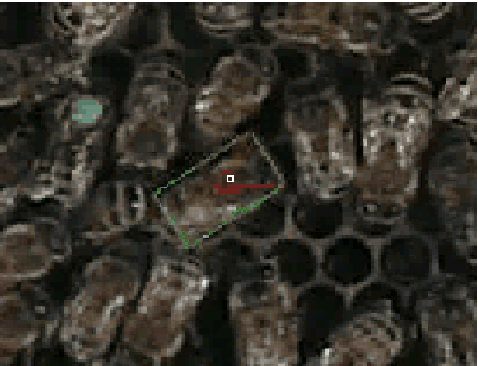
\includegraphics[width=0.23\linewidth]{changepoints/figs/app/tracker-1.png} \hspace{2em}
    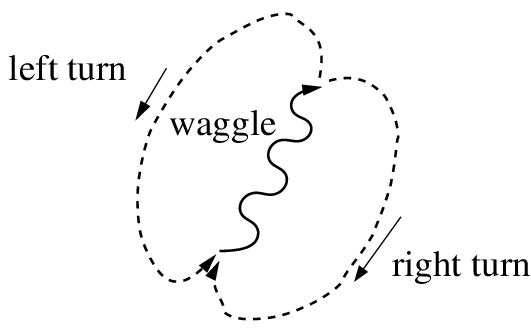
\includegraphics[width=0.27\linewidth]{changepoints/figs/app/bee_dance-1.png}
\caption{Dancer bees are tracked by a appearance based tracker from video sequences. The tracked bee is shown in green rectangle in the left figure above. The right figure shows a stylized bee dance through which bees talk to the other bees about the orientation and distance to the food sources.}
\label{fig:bees}
\end{figure}

\begin{figure}[H]
    \centering
    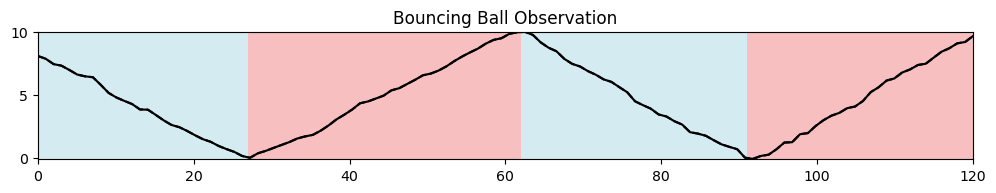
\includegraphics[width=0.85\linewidth]{changepoints/figs/ex/ex0.png}
    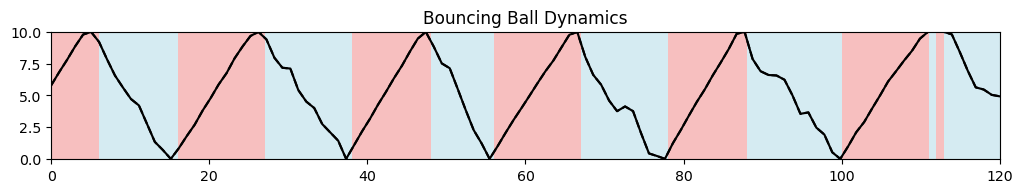
\includegraphics[width=0.85\linewidth]{changepoints/figs/ex/ex1.png}
    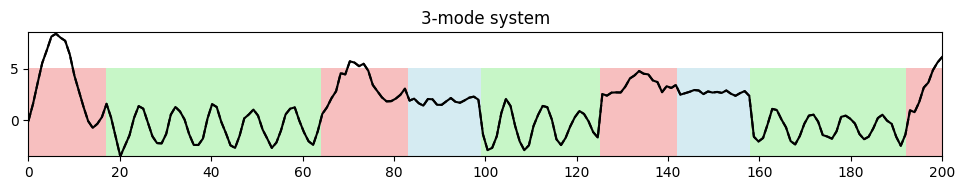
\includegraphics[width=0.85\linewidth]{changepoints/figs/ex/ex2.png}
    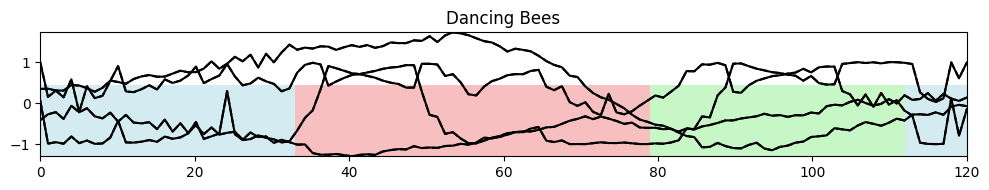
\includegraphics[width=0.85\linewidth]{changepoints/figs/ex/ex3.png}
    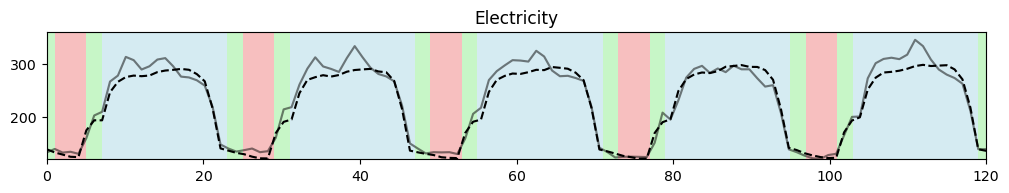
\includegraphics[width=0.85\linewidth]{changepoints/figs/ex/ex4.png}
    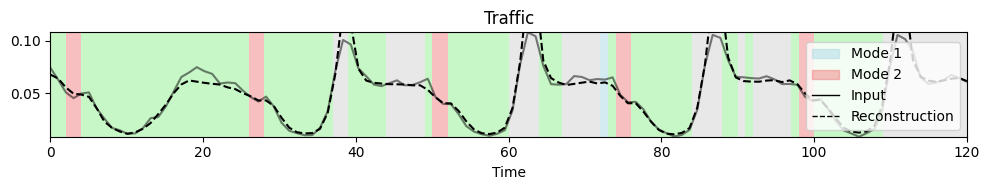
\includegraphics[width=0.85\linewidth]{changepoints/figs/ex/ex5.png}
\caption{Examples of datasets and prediction results. Dotted line represents prediction whereas solid lines represents ground truth; background colors
represent the different operating modes segmented by our base predictor RED-SDS.}
\label{fig:examples}
\end{figure}

\newpage
\subsection{Additional Experiments}
\label{app:more_experiments}

\paragraph{Additional Baselines} We add comparison to three more baselines that handles distribution shift in time series data. They are DtACI \cite{angelopoulos2024online},  ECI \cite{wu2025error}, and L-ARC \cite{zecchin2024localized}.

We would like to emphasize that these baselines are reactive. The question we try to address with CPTC is - what happens when we can anticipate distribution shift? CPTC is designed such that it greatly improves coverage compared to purely reactive methods, while still maintaining the ability to adapt to unknown shifts. To our knowledge, there are no other models that explore the same problem; CPTC provides practitioners with a simple and sound solution, when they have the ability (such as via a state space model) to predict shifts.

\begin{table}[h]
\caption{Performance on synthetic and real-world datasets with target confidence $1-\alpha = 0.9$ (for horizon $T=200$ for synthetic datasets, $300$ for electricity and traffic, and $60$ for bee, mean $\pm$ standard deviation of the test samples).  Methods that are \textit{invalid} (coverage below $90\%$) are grayed out. Our method achieves a high level of calibration (coverage is close to $90\%$) consistently. }
\vspace{1em}
\label{tab:baselines}
\centering
\resizebox{0.8\textwidth}{!}{%
\begin{tabular}{ l | c | c  c c c } 
\toprule
& & DtACI & ECI-cutoff & L-ARC & Ours \\ 
\midrule\midrule
\multirow{2}{*}{\begin{tabular}{l}Bouncing  \\ Ball obs.\end{tabular}} & Cov & \color{gray}{82.97 \plusminus 1.35}& \color{gray}{79.86 \plusminus 1.42}& \color{gray}{75.12 \plusminus 9.25} & 92.06 \plusminus 1.93\\ 
 & Width & \color{gray}{3.21 \plusminus 0.80}& \color{gray}{3.02 \plusminus 0.72}& \color{gray}{1.89 \plusminus 0.76} & 10.70 \plusminus 3.01\\ 
\midrule
\multirow{2}{*}{\begin{tabular}{l}Bouncing  \\ Ball dyn.\end{tabular}} & Cov & \color{gray}{79.63 \plusminus 1.10}& \color{gray}{80.91 \plusminus 1.28}& \color{gray}{78.63 \plusminus 6.21} & 90.62 \plusminus 3.85\\ 
 & Width & \color{gray}{3.51 \plusminus 2.20}& \color{gray}{2.32 \plusminus 0.19}& \color{gray}{2.44 \plusminus 0.23} & 10.73 \plusminus 3.67\\ 
\midrule
\multirow{2}{*}{\begin{tabular}{l}3-Mode \\ System\end{tabular}} & Cov & \color{gray}{88.82 \plusminus 0.95}& \color{gray}{83.67 \plusminus 0.89}& 92.58 \plusminus 2.77 & 90.43 \plusminus 1.92\\ 
 & Width & \color{gray}{12.55 \plusminus 7.52}& \color{gray}{2.39 \plusminus 0.48}& 12.31 \plusminus 2.85 &  4.80 \plusminus 2.64\\ 
\midrule
\midrule
\multirow{2}{*}{\begin{tabular}{l}Traffic\end{tabular}} & Cov & \color{gray}{89.14 \plusminus 0.40}& \color{gray}{86.12 \plusminus 0.50}& 90.05 \plusminus 6.24 & 92.38 \plusminus 1.24\\ 
 & Width & \color{gray}{10.35 \plusminus 9.85}& \color{gray}{7.02 \plusminus 9.72}& 8.39 \plusminus 10.13 & 15.83 \plusminus 5.96\\ 
\midrule
\multirow{2}{*}{\begin{tabular}{l}Electricity\end{tabular}} & Cov & \color{gray}{88.35 \plusminus 0.38}& \color{gray}{89.41 \plusminus 0.47}& \color{gray}{86.42 \plusminus 4.96} & 91.19 \plusminus 1.22\\ 
 & Width & \color{gray}{189.51 \plusminus 187.25}& \color{gray}{138.72 \plusminus 83.30}& \color{gray}{157.82 \plusminus 95.02} & 249.46 \plusminus 1365.46 \\ 
\midrule
\multirow{2}{*}{\begin{tabular}{l}Dancing \\ Bees\end{tabular}} & Cov & \color{gray}{78.91 \plusminus 3.02}& \color{gray}{80.12 \plusminus 2.85}& \color{gray}{75.92 \plusminus 14.21} & 95.71 \plusminus 4.95 \\
 & Width & \color{gray}{0.03 \plusminus 0.01}& \color{gray}{0.08 \plusminus 0.01}& \color{gray}{0.28 \plusminus 0.15} & 0.33 \plusminus 0.14 \\
\bottomrule
\end{tabular}
}
\end{table}

\paragraph{Longer horizon Data} Result for the same set of experiments performed on longer horizon  ($T=10,000$ for synthetic datasets amd $T=4,000$ for Electricity and Traffic datasets) is presented in table \ref{tab:baselines_long_horizon}. We added the setting where the added noise to the bouncing ball dataset is varying over the course of the time series, which is more challenging than the original settings. In the longer horizon case, both SPCI and HopCPT achieve their state of the art performance. Our method remains valid yet achieves less sharp interval width. 

\begin{table}[H]
\caption{Longer time horizon ($T=10,000$ for synthetic datasets amd $T=4,000$ for Electricity and Traffic datasets). Performance in synthetic and real-world datasets with target confidence $1-\alpha = 0.9$. Methods that are \textit{invalid} (coverage below $90\%$) are grayed out. Our method achieves a high level of calibration (coverage is close to $90\%$) consistently.} \vspace{0.5em}
\label{tab:baselines_long_horizon}
\centering
\resizebox{\textwidth}{!}{%
\begin{tabular}{ l | c | c  c c c c c }\toprule
& & RED-SDS & CP & ACI & SPCI  & HopCPT & Ours \\
\midrule\midrule
\multirow{2}{*}{\begin{tabular}{l}Bouncing Ball \\ obs.\end{tabular}} & Cov & \color{gray}{89.31 \plusminus 5.15}& \color{gray}{81.55 \plusminus 7.10} & 89.25 \plusminus 1.40 & 90.05 \plusminus 0.04 & 90.02 \plusminus 0.02 & 90.53 \plusminus 0.23\\
 & Width & \color{gray}{2.65 \plusminus 0.11}& \color{gray}{2.65 \plusminus 0.85}& 3.53 \plusminus 0.81& 1.95 \plusminus 0.12 & 1.99 \plusminus 0.08 & 2.25 \plusminus 0.54\\
\midrule
\multirow{2}{*}{\begin{tabular}{l}Bouncing Ball \\ dyn.\end{tabular}} & Cov & \color{gray}{45.12 \plusminus 25.50}& \color{gray}{42.88 \plusminus 6.95}& \color{gray}{87.95 \plusminus 1.05}& 90.04 \plusminus 0.04 & 90.01 \plusminus 0.04 & 90.05 \plusminus 0.04\\
 & Width & \color{gray}{1.67 \plusminus 0.13}& \color{gray}{0.95 \plusminus 0.51}& \color{gray}{3.10 \plusminus 1.04}& 3.24  \plusminus 0.14 & 3.07 \plusminus 0.10 & 3.18 \plusminus 0.91\\
\midrule
\multirow{2}{*}{\begin{tabular}{l}3-Mode \\ System\end{tabular}} & Cov & \color{gray}{68.52 \plusminus 3.53}& \color{gray}{65.24 \plusminus 5.51}& 89.75 \plusminus 0.90& 90.05 \plusminus 0.02 & 90.02 \plusminus 0.04 & 90.08 \plusminus 0.05\\
 & Width & \color{gray}{2.56 \plusminus 0.21}& \color{gray}{2.33 \plusminus 0.63}& 3.74 \plusminus 0.61& 2.67 \plusminus 0.94 & 2.49 \plusminus 1.31 &  3.12 \plusminus 2.63\\
\midrule
\midrule
\multirow{2}{*}{\begin{tabular}{l}Bouncing Ball \\ obs. varying\end{tabular}} & Cov & \color{gray}{60.83 \plusminus 22.53}& \color{gray}{40.25 \plusminus 6.52}& 88.60 \plusminus 1.25& 90.02 \plusminus 0.04 & 90.04 \plusminus 0.00 & 90.10 \plusminus 0.03\\
 & Width & \color{gray}{2.10 \plusminus 0.45}& \color{gray}{1.73 \plusminus 0.91}& 3.70 \plusminus 0.95 & 2.11 \plusminus 0.82 & 2.14 \plusminus 0.73 & 2.41 \plusminus 1.22\\
\midrule
\multirow{2}{*}{\begin{tabular}{l}Bouncing Ball \\ dyn. varying\end{tabular}} & Cov & \color{gray}{44.25 \plusminus 26.11}& \color{gray}{41.73 \plusminus 7.12}& \color{gray}{88.05 \plusminus 1.00}& 90.05 \plusminus 0.03 & 90.02 \plusminus 0.04 & 90.08 \plusminus 0.03\\
 & Width & \color{gray}{1.85 \plusminus 0.12}& \color{gray}{0.92 \plusminus 0.55}& \color{gray}{3.13 \plusminus 1.14}& 2.92 \plusminus 0.21 & 3.05 \plusminus 0.19 & 3.40 \plusminus 0.32\\
\midrule
\midrule
\multirow{2}{*}{\begin{tabular}{l}Traffic\end{tabular}} & Cov & \color{gray}{87.14 \plusminus 10.51}& \color{gray}{70.52 \plusminus 2.83}& \color{gray}{89.15 \plusminus 0.38}& 90.01 \plusminus 0.04 & 90.03 \plusminus 0.03 & 90.02 \plusminus 0.03\\
 & Width & \color{gray}{2.91 \plusminus 1.62}& \color{gray}{0.43 \plusminus 0.25}& \color{gray}{55.10 \plusminus 24.13}& 4.81 \plusminus 2.42 & 7.84 \plusminus 10.53 & 8.55 \plusminus 14.11\\
\midrule
\multirow{2}{*}{\begin{tabular}{l}Electricity\end{tabular}} & Cov & \color{gray}{76.10 \plusminus 13.52}& \color{gray}{69.53 \plusminus 3.21}& \color{gray}{89.05 \plusminus 0.33}& 90.02 \plusminus 0.03 & 90.00 \plusminus 0.02 & 90.43 \plusminus 0.03\\
 & Width & \color{gray}{91.30 \plusminus 125.10}& \color{gray}{62.10 \plusminus 451.20}& \color{gray}{31.40 \plusminus 171.30}& 162.02 \plusminus 11.40 & 161.70 \plusminus 15.20 & 173.38 \plusminus 31.10 \\
\bottomrule
\end{tabular}
}
\end{table}

\paragraph{Aggregation methods.} In this study we compare the two different aggregation methods. First is the case where we chose the minimum size, i.e. $\Gamma_t(x_t) = $ \Eqref{eq:aggregation-average}. Algorithmically, we discretize the output space $\mathcal{Y}$ into intervals of length 0.02, and calculate probability mass for each interval. We refer to this method as \emph{min}. Aggregation by union numbers (the same as in the main text using \Eqref{eq:aggregation-union}) are referred to as \emph{union}. Results are present in table \ref{tab:aggregation} where the performance are very similar. When there are two modes (bouncing ball cases) the prediction intervals are almost identical.
 
\begin{table}[h!]
\centering
\caption{Ablation Study on two different Union (\textit{union}, \eqref{eq:aggregation-union}) and grid-discretization (\textit{min}, \eqref{eq:aggregation-average}).}
\vspace{0.5em}
\label{tab:aggregation}
\begin{tabular}{lcccccc}
\toprule
& BB obs. & BB dyn. & 3-mode system & traffic & electricity & bees \\
\midrule
\midrule
Coverage (\textit{union}) & 90.53 & 90.44 & 93.35 & 92.76 & 92.62 & 93.43 \\
Coverage (\emph{min})  & 90.03 & 90.32 & 91.50 & 91.87 & 89.82 & 90.28 \\
Width (\textit{union})   & 3.73  & 1.72  & 2.45 & 7.94  & 166.88 & 0.79 \\
Width (\emph{min})     & 3.62 & 1.65  & 2.41 & 7.95  & 153.57 & 0.77 \\
\bottomrule
\end{tabular}
\end{table}

\paragraph{Discussion on Misspecified Regimes.} We designed the number of latent states to be a hyperparameter given by the user. Our method ensures that the validity guarantee still holds even if the state cardinality is incorrect (theorem 4.2), as incorrect state cardinality can be formulated as a case of incorrect classification. Determining state space cardinality is a well-studied problem (see for example \cite{branicky1994stability}), and we consider it to be beyond the scope of our paper.

Regarding the effect on performance, our ablation studies (Section 5.2, Tables \ref{tab:z_exp} and \ref{tab:z_exp_area}) demonstrate that while the validity (coverage) of CPTC is robust to errors in state prediction, the sharpness (width of prediction intervals) can be affected. Table 3 explicitly shows that "the more accurate the state prediction is, the sharper the intervals." This implies that selecting a more appropriate number of regimes that better captures the true underlying dynamics would lead to narrower and more efficient prediction intervals.

\subsection{Qualitative Results}
\label{app:pictures}

We provide additional visualizations to present qualitative comparisons of CPTC compared to baseline models. Figures \ref{fig:synthetic}, \ref{fig:pic2}, and \ref{fig:pic3} show consistent results with the analysis in section 5, where CPTC shows stronger adaptivity and validity for uncertainty quantification in time series with these nonstationary dynamics.



\begin{figure}[h!]
    \centering
    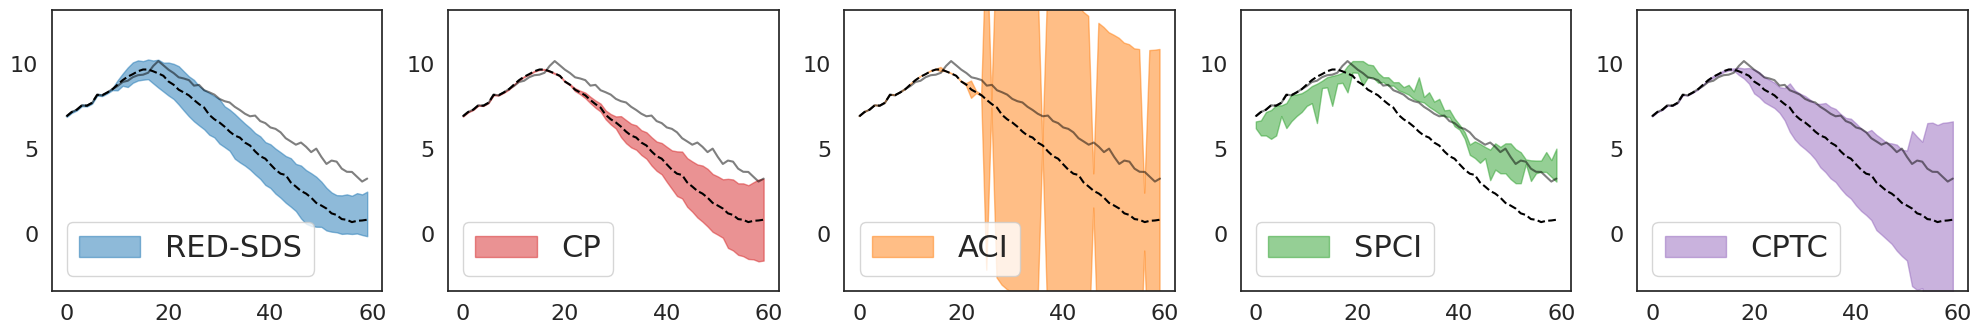
\includegraphics[width=\linewidth]{changepoints/figs/ex/a.png}
    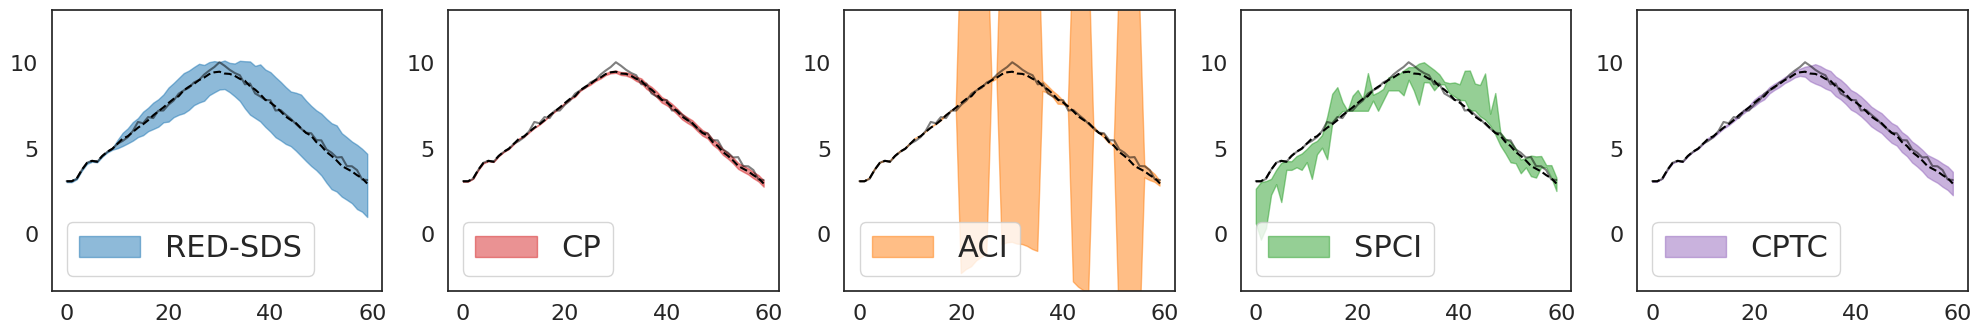
\includegraphics[width=\linewidth]{changepoints/figs/ex/b.png}
    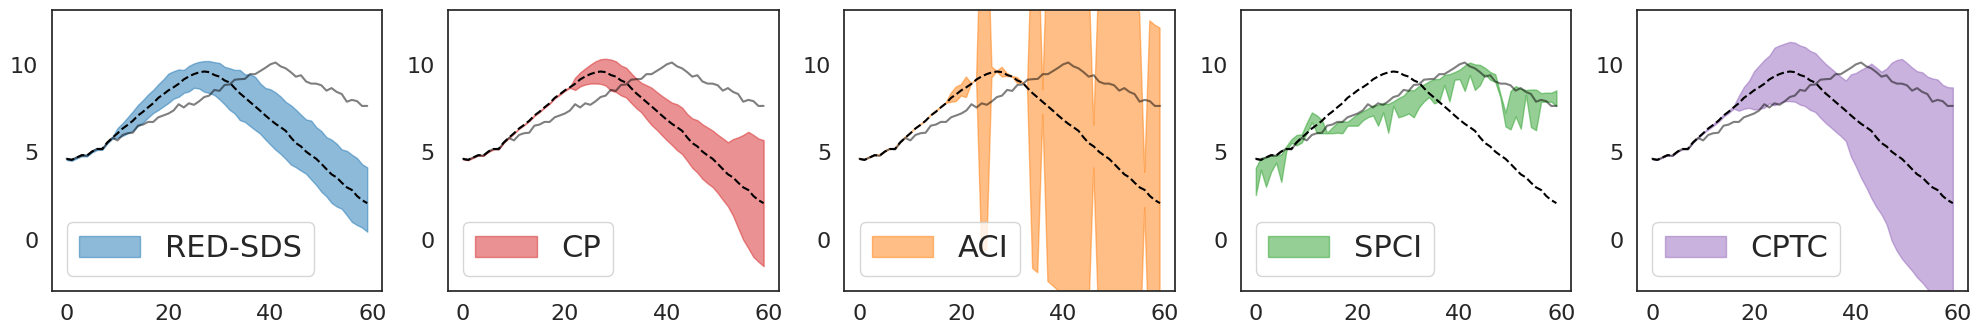
\includegraphics[width=\linewidth]{changepoints/figs/ex/c.png}
    \caption{\textbf{Qualitative comparison of the prediction interval on the bouncing ball w/ dynamics noise dataset.} The dashed line is the predicted state whereas the solid gray line is the observation. We see that our CPTC algorithm can increase the interval in anticipation of an uncertain state change (top panel), is stabler when the prediction is accuracy compared to ACI and SPCI (middle panel), and is adaptive to inaccurate predictions (botom panel).}
    \label{fig:synthetic}
     %\vspace{-0.5em}
\end{figure}


% \begin{figure}[H]
%     \centering
%     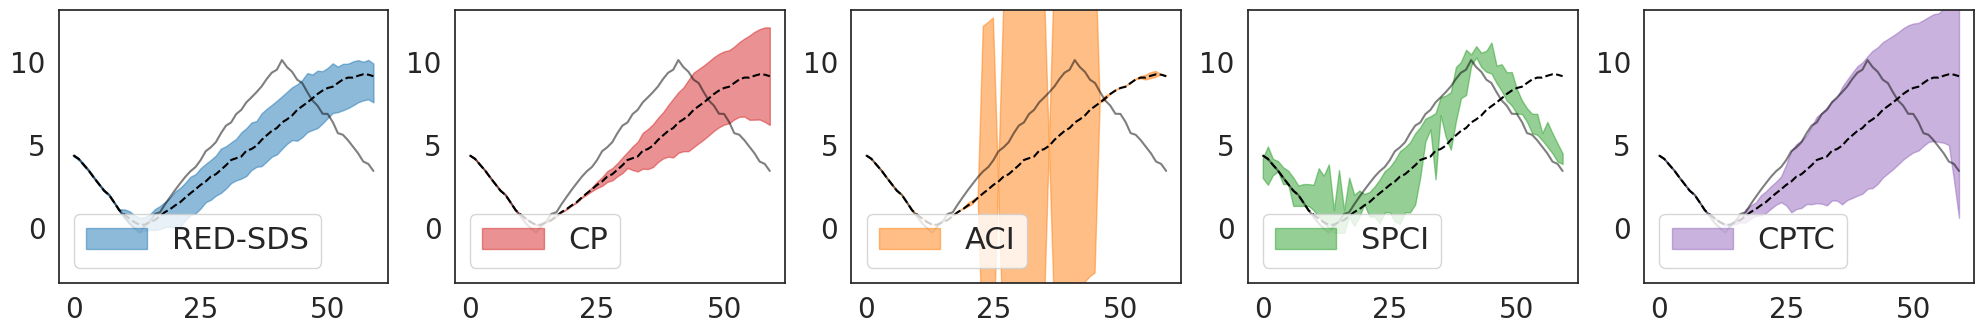
\includegraphics[width=\linewidth]{changepoints/figs/app/a1.png}
%     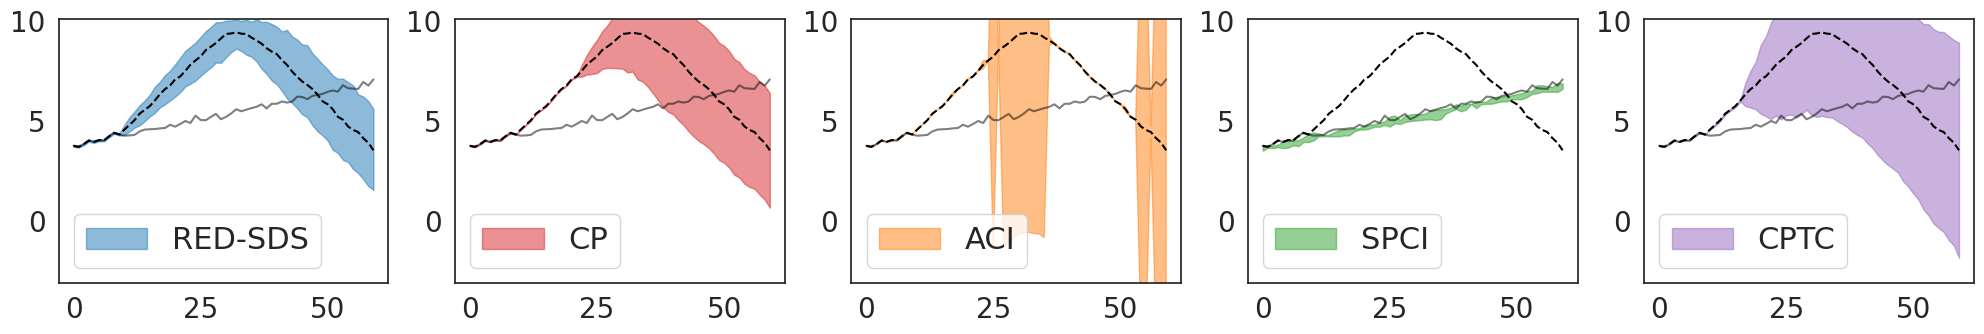
\includegraphics[width=\linewidth]{changepoints/figs/app/a2.png}
%     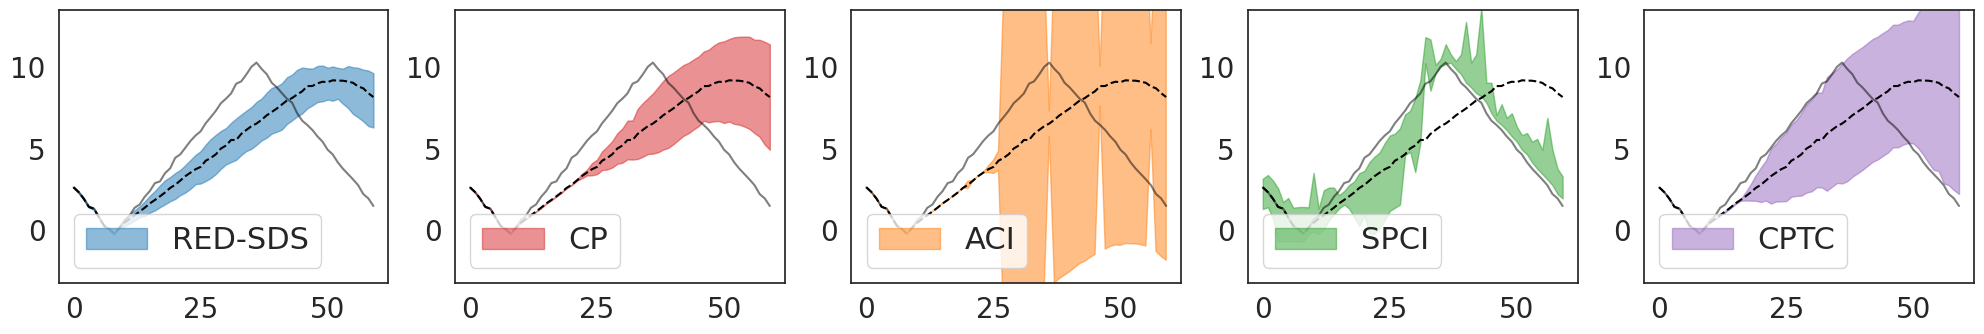
\includegraphics[width=\linewidth]{changepoints/figs/app/a3.png}
%     \caption{Visualization of prediction intervals on the Bouncing Ball Obs dataset.}
%     \label{fig:pic1}
%     \vspace{-1em}
% \end{figure}
\vspace{-1em}
\begin{figure}[H]
    \centering
    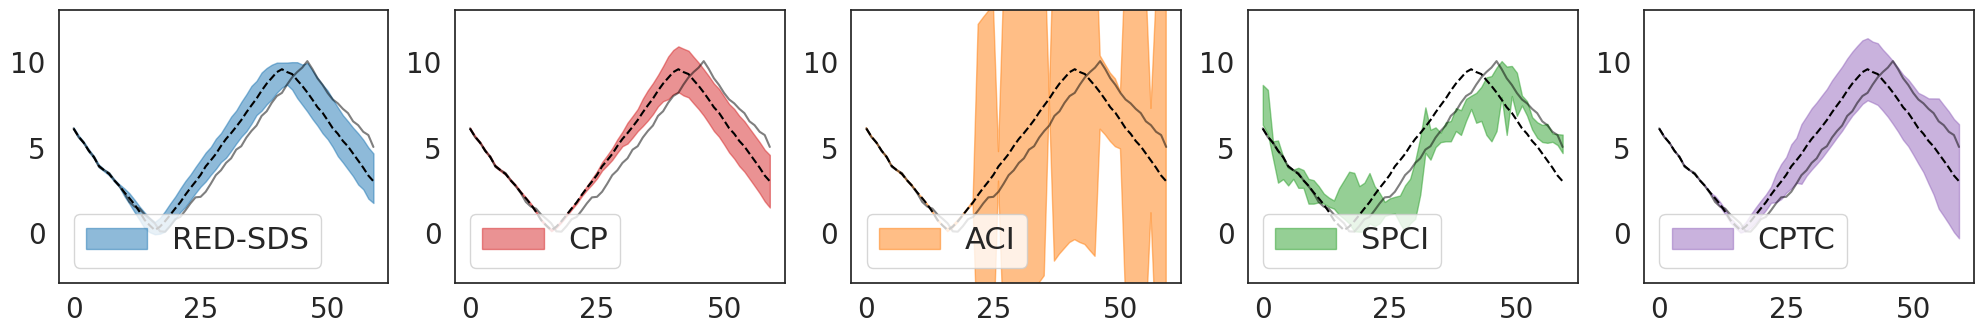
\includegraphics[width=\linewidth]{changepoints/figs/app/b1.png}
    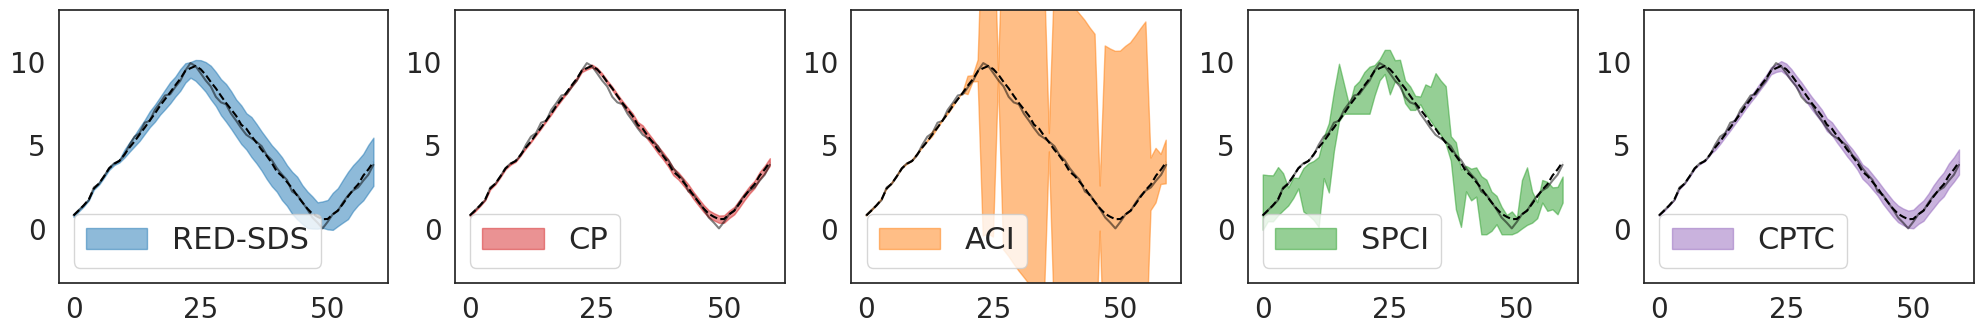
\includegraphics[width=\linewidth]{changepoints/figs/app/b2.png}
    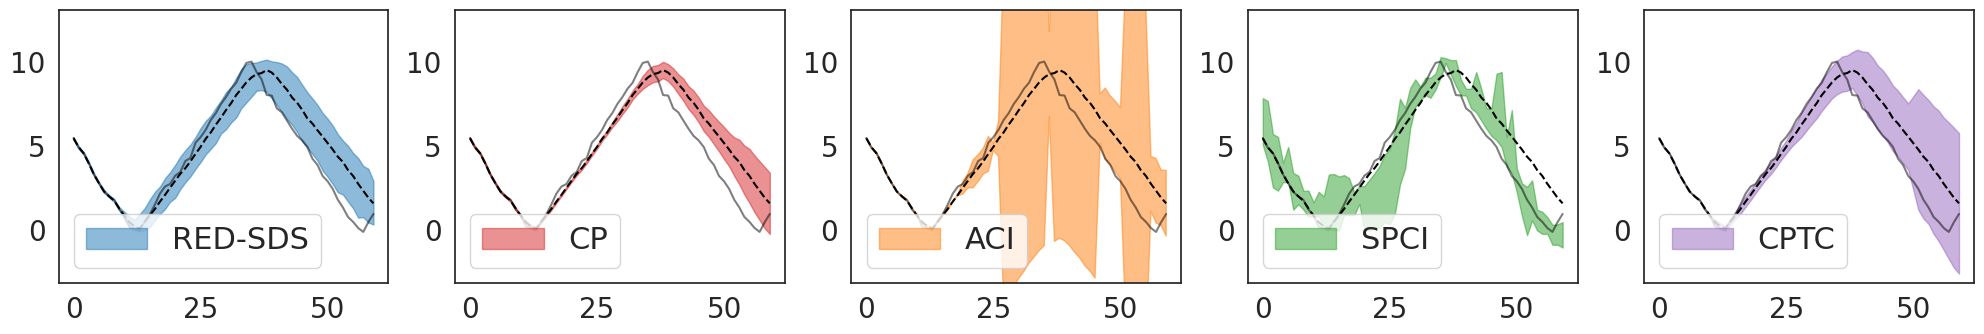
\includegraphics[width=\linewidth]{changepoints/figs/app/b3.png}
    \caption{Visualization of prediction intervals on the Bouncing Ball Obs dataset.}
    \label{fig:pic2}
\end{figure}
\vspace{2em}

\begin{figure}[H]
    \centering
    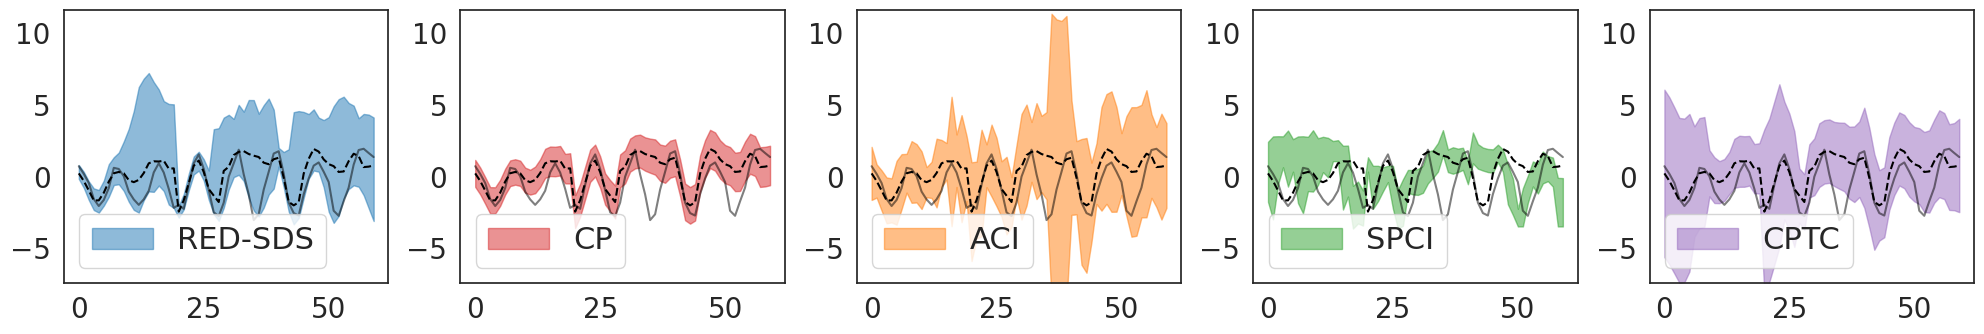
\includegraphics[width=\linewidth]{changepoints/figs/app/c1.png}
    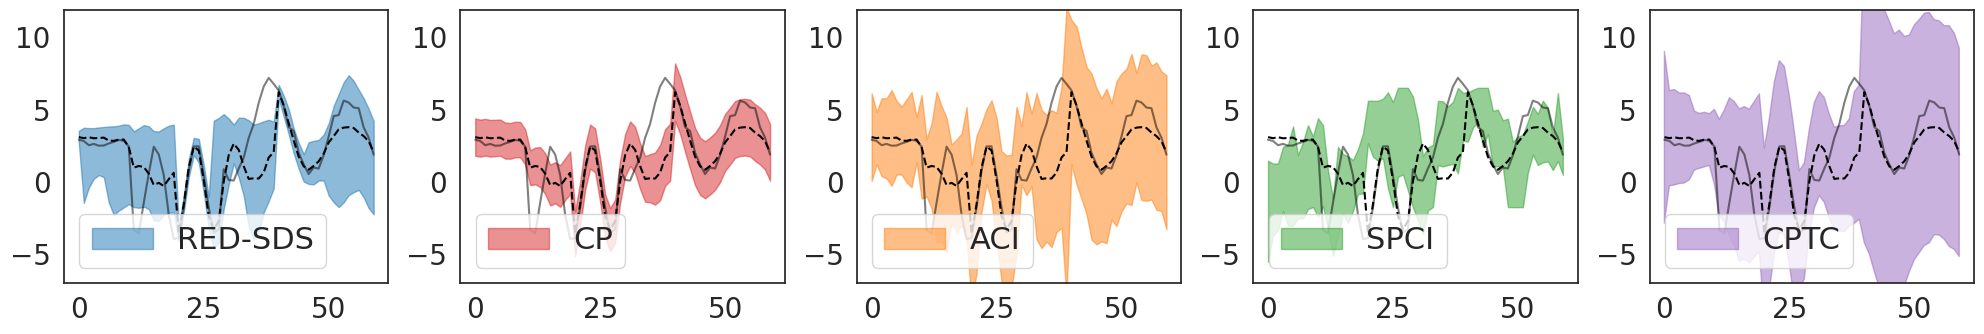
\includegraphics[width=\linewidth]{changepoints/figs/app/c2.png}
    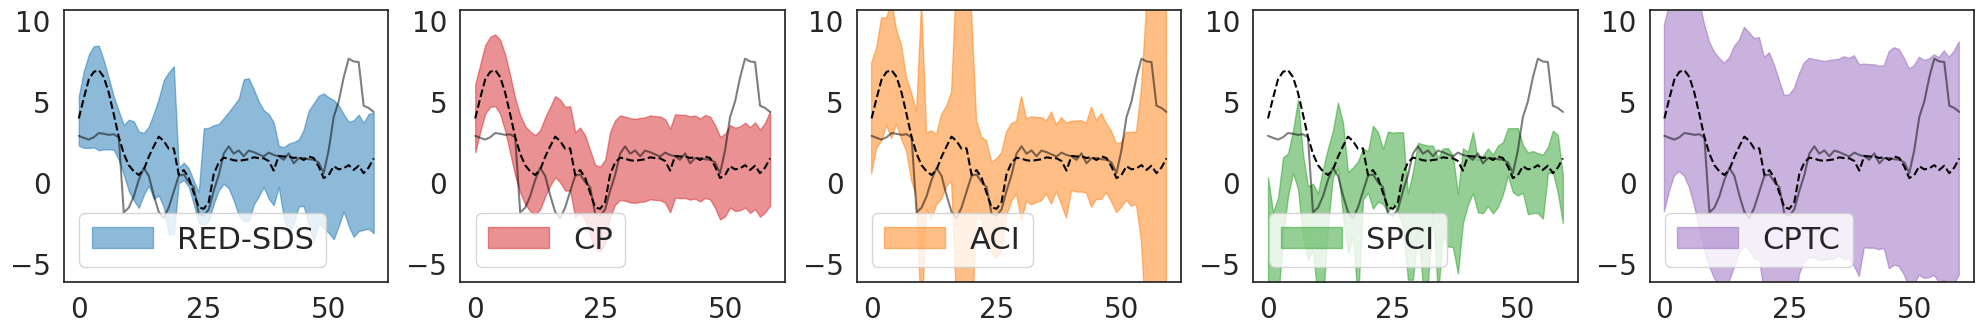
\includegraphics[width=\linewidth]{changepoints/figs/app/c3.png}
    \caption{Visualization of prediction intervals on the 3 mode system datasets.}
    \label{fig:pic3}
\end{figure}

\section{Runtime analysis}

We provide a runtime analysis comparing the aggregation methods in Equations \ref{eq:aggregation-average} and \ref{eq:aggregation-union} and with baselines.

\textbf{Notation}

\begin{itemize}
    \item $T$: Total timesteps, $K$: Number of states, $M$: State prediction model inference complexity
    \item Score sets $\mathcal{S}_z$ maintained in sorted order (quantile computation in $\mathcal{O}(1)$, insertion $\mathcal{O}(\log T)$)
\end{itemize}

\textbf{Complexity Per Timestep}

\begin{enumerate}
    \item Computing quantile $Q^{1-\alpha_t}(\mathcal{S}_z^{(l)})$ for each state, totaling $\mathcal{O}(K)$.
    \item State Prediction: computing $\hat{p}(z_t|x_t)$ and sampling a state, totaling $\mathcal{O}(M)$.
    \item Aggregation
    \begin{itemize}
        \item \textit{Eq. 10, Weighted Level-Set:} $\mathcal{O}(K \cdot \lceil 1/\delta \rceil^d)$ where $\delta$ is discretization resolution
        \item \textit{Eq. 11, Union:} $\mathcal{O}(K \log K)$ for sorting states by probability
    \end{itemize}
    \item Updates: $\mathcal{O}(\log t)$ for inserting new score into sorted set.
\end{enumerate}

\textit{Therefore, the total complexity of CPTC with horizon $T$ is:}

$\mathcal{O}(T \cdot (M + K \cdot \lceil \frac{1}{\delta} \rceil^d) + T \log T)$ if we use the Weighted Level-Set as aggregation in Eq. 10, and

$\mathcal{O}(T \cdot (M + K \log K) + T \log T)$ if we use the more efficient Union aggregation in Eq. 11.

In practice, both $M$ (inference cost) and $K$ (number of discrete states) are small. For applications where $K = \mathcal{O}(1)$ and $M = \mathcal{O}(1)$, CPTC achieves near-linear scaling $\mathcal{O}(T \log T)$, the same as ACI (see table below).

If we use the more precise weighted level set aggregation method, the runtime largely depends on the discretization resolution $\delta$, output dimension $d$, and the number of states $K$. We remark the level set approach scales poorly if the resolution, dimension, or number of states are high.

\begin{table}[h]
\centering
\begin{tabular}{lll}
\hline
\textbf{Method} & \textbf{Time Complexity} & \textbf{Remarks} \\
\hline
ACI & $\mathcal{O}(T \log T)$ & Single score set, no state awareness \\
SPCI / HopCPT & $\mathcal{O}(T^2 \log T)$ & Re-train regression model at every time step \\
CPTC (Union) & $\mathcal{O}(T \log T)$ & State-aware, pre-trained predictor \\
\hline
\end{tabular}
\end{table}
% \subsection{Ablation study on non state-dependent forecaster}

% We can still use CPTC when we only have one forecaster but have access to some state prediction (for example in the form of external parameters). We can apply algorithm \ref{alg:cptc} directly with the special case where $\hat{f}(x,z_i) = \hat{f}(x,z_j)$ for any $x \in \gX and z_i, z_j \in \gZ$. Table \ref{tab:one_forecaster} presents the performance of the algorithm in this case.

% \begin{table}[]
% \caption{One forecaster} %\vspace{-0.5em}
% \label{tab:one_forecaster}
% \centering
% \begin{tabular}{ l | c | c  c } 
% \toprule
% & & SPCI  & Ours \\
% \midrule\midrule
% \multirow{2}{*}{\begin{tabular}{l}Bouncing Ball \\ obs.\end{tabular}} & Cov & \color{gray}{37.90 \plusminus 9.78} & 92.16 \plusminus 26.88\\ 
%  & Width & \color{gray}{1.45 \plusminus 0.85} & 7.43 \plusminus 4.68\\ 
% \midrule
% \multirow{2}{*}{\begin{tabular}{l}Bouncing Ball \\ dyn.\end{tabular}} & Cov & \color{gray}{53.62 \plusminus 7.75} & 90.58 \plusminus 29.21\\ 
%  & Width & \color{gray}{2.02 \plusminus 0.23} & 8.11 \plusminus 4.93\\ 
% \midrule
% \multirow{2}{*}{\begin{tabular}{l}3-Mode \\ System\end{tabular}} & Cov & \color{gray}{81.72 \plusminus 2.88} & 93.35 \plusminus 3.51\\ 
%  & Width & \color{gray}{3.94 \plusminus 0.85} & 13.68 \plusminus 2.49\\ 
% \midrule\midrule
% \multirow{2}{*}{\begin{tabular}{l}Traffic\end{tabular}} & Cov & \color{gray}{88.24 \plusminus 2.13} & 94.76 \plusminus 4.93\\ 
%  & Width & \color{gray}{4.62 \plusminus 2.28} & 8.34 \plusminus 14.44\\ 
% \midrule
% \multirow{2}{*}{\begin{tabular}{l}Electricity\end{tabular}} & Cov & \color{gray}{86.62 \plusminus 2.97} & 93.82 \plusminus 4.22\\ 
%  & Width & \color{gray}{371.69 \plusminus 305.86} & 98.87 \plusminus 49.35\\ 
% \midrule
% \multirow{2}{*}{\begin{tabular}{l}Dancing Bees\end{tabular}} & Cov & \color{gray}{79.2 \plusminus 0.3} & 93.43 \plusminus 11.42 \\
%  & Width & \color{gray}{1.77 \plusminus 1.38} & 1.15 \plusminus 0.56 \\
% \bottomrule
% \end{tabular}
% \end{table}



% \subsection{Experiment on state prediction (continued) }
% \label{app:z_exp}

% \begin{table*}[h!]
%     \centering
%     \begin{tabular}{c|c c c c}
%         \hline
%         \toprule
%         $T=250$& Ground truth state labels & GT w/ $20\%$ error & GT w/ $50\%$ error & Learned state labels \\ 
%         \midrule
%         BB obs. noise & 90.00 \plusminus 0.32 & 89.94 \plusminus 0.29 & 89.92 \plusminus 0.28 & 89.11 \plusminus 3.54 \\ 
%         BB dyn. noise & 90.04 \plusminus 0.34 & 90.01 \plusminus 0.35 & 89.96 \plusminus 0.30 & 90.11 \plusminus 0.33\\ 
%         3-mode system & 89.34 \plusminus 0.87 &  89.40 \plusminus 0.91  & 89.64 \plusminus 0.80 & 89.72 \plusminus 1.51 \\ 
%         \midrule\midrule
%         $T=1000$& Ground truth state labels & GT w/ $20\%$ error & GT w/ $50\%$ error & Learned state labels \\ 
%         \midrule
%         BB obs. noise & 90.00 \plusminus 0.32 & 89.94 \plusminus 0.29 & 89.92 \plusminus 0.28 & 89.11 \plusminus 3.54 \\ 
%         BB dyn. noise & 90.04 \plusminus 0.34 & 90.01 \plusminus 0.35 & 89.96 \plusminus 0.30 & 90.11 \plusminus 0.33\\ 
%         3-mode system & 89.34 \plusminus 0.87 &  89.40 \plusminus 0.91  & 89.64 \plusminus 0.80 & 89.72 \plusminus 1.51 \\ 
%         \bottomrule
%     \end{tabular}
%     \caption{Coverage of CPTC for using ground truth (GT) labels, GT labels with injected noise, and learned  label predictions on synthetic data with $T=250, 1000$. We can see that coverage performance does not change significantly with error in state prediction. }
%     \label{tab:z_exp_small}
% \end{table*}